\chapter{System's architecture}
\label{chap1}
\section{IP Manager interfaces}
\lhead{Disclaimer, this was done by project 13'members Authors: Floridia, Margelli, Mocerino, Ngongang}
A multi IP-core system requires a IP core manager to handle the complexity of this system.
Main tasks of the IP Manager are the correct selection of the target IP and the interrupt handling. Figure \ref{00fig} shows the overall architecture of the whole system. 
	\begin{figure}[h]
		\centering
		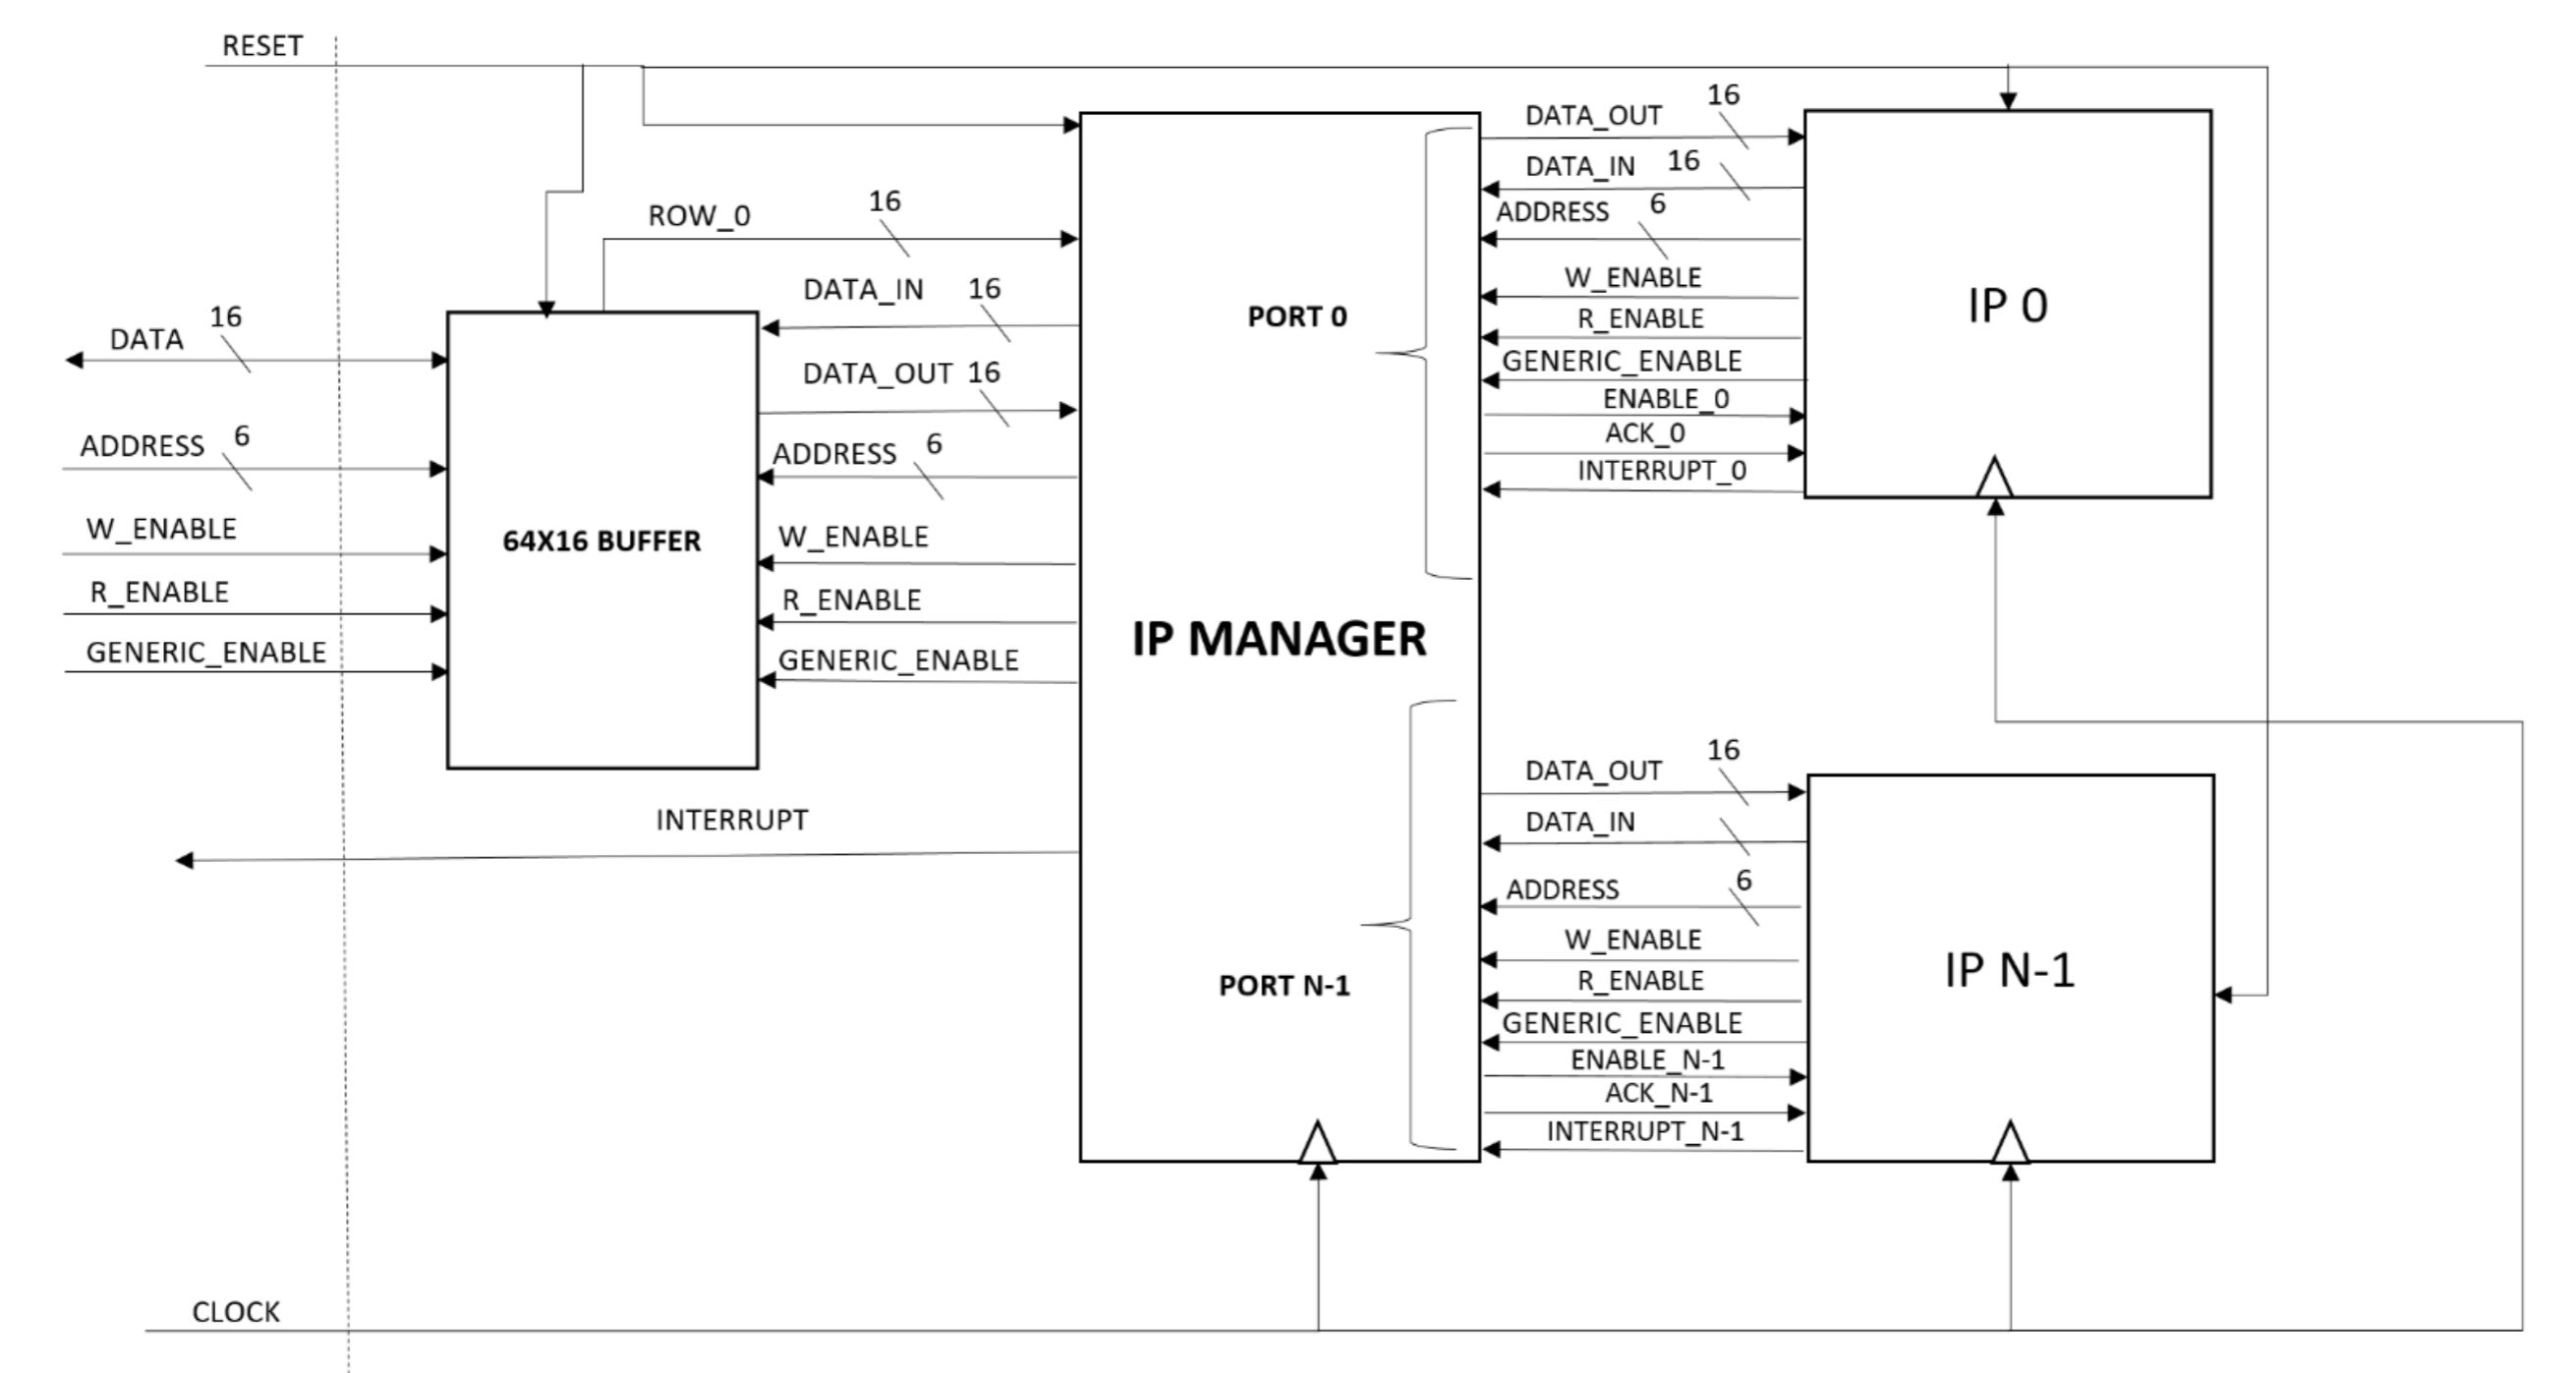
\includegraphics[width=\textwidth]{chapters/figures/00.png}  
		\caption{System architecture}
		\label{00fig}
	\end{figure}
	
	As shown in the figure, the IP manger has a standard interface with the buffer. This interface is used to redirect data to/from the target IP and to access the buffer itself (e.g. to write the row 0).\\ However, it is
	provided with a direct access (read-only) to the internal element to speed-up the routing process whenever a new transaction begins. It is important to underline that for each instantiated IP there are a set ofstandard signals and some protocol-specific signals. The former are the very same signals used for accessing the buffer, whilst the latter are used for handling interrupt requests. For sake of clarity, we report the function of the IP-specific signals for the generic IP x:
